\begin{figure}[t]%
  \captionsetup[subfloat]{justification=RaggedLeft,singlelinecheck=false}
    \centering
    \subfloat[\\Band-doubling\\(\edlib)]{
\includegraphics[width=0.33\linewidth]{imgs/intro/1_ukkonen.png}\label{fig1-band}}
    \hspace{-8em}
    \hfill
    \subfloat[\\\dijkstra] {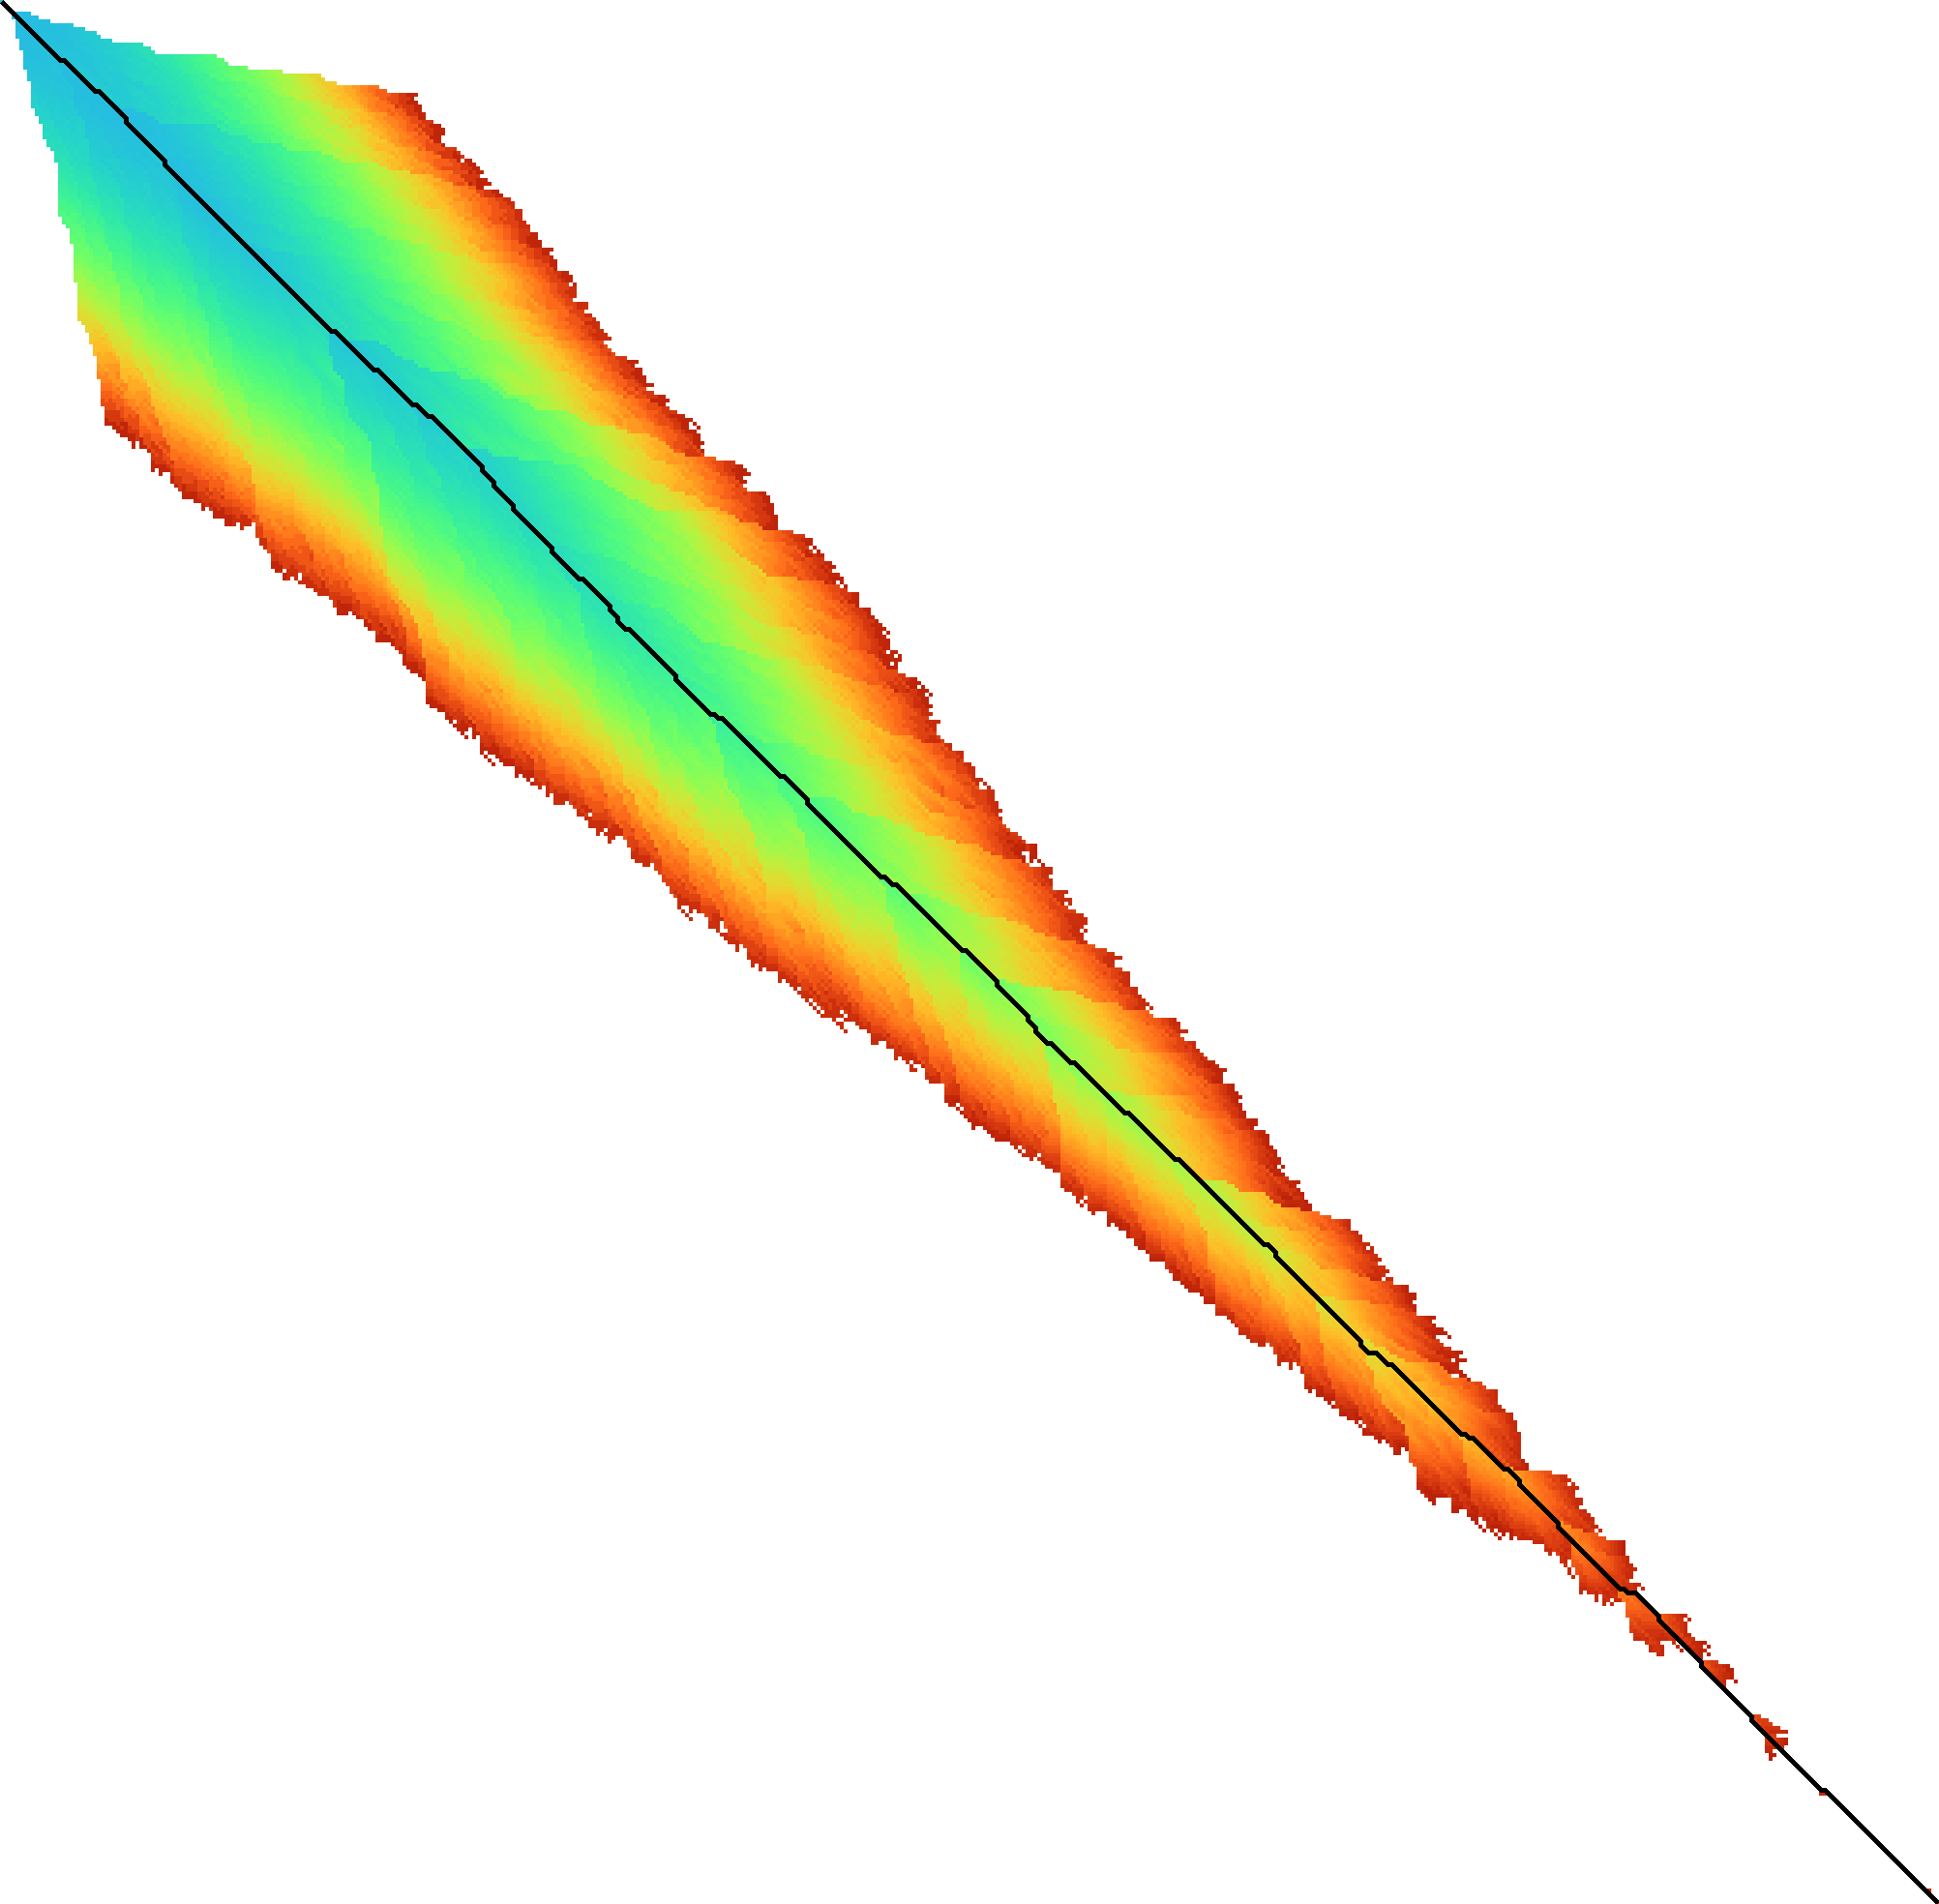
\includegraphics[width=0.33\linewidth]{imgs/intro/2_dijkstra.png}\label{fig1-dij}}
    \hspace{-8em}
    \hfill
    \subfloat[\\DT\\(\oldwfa)]{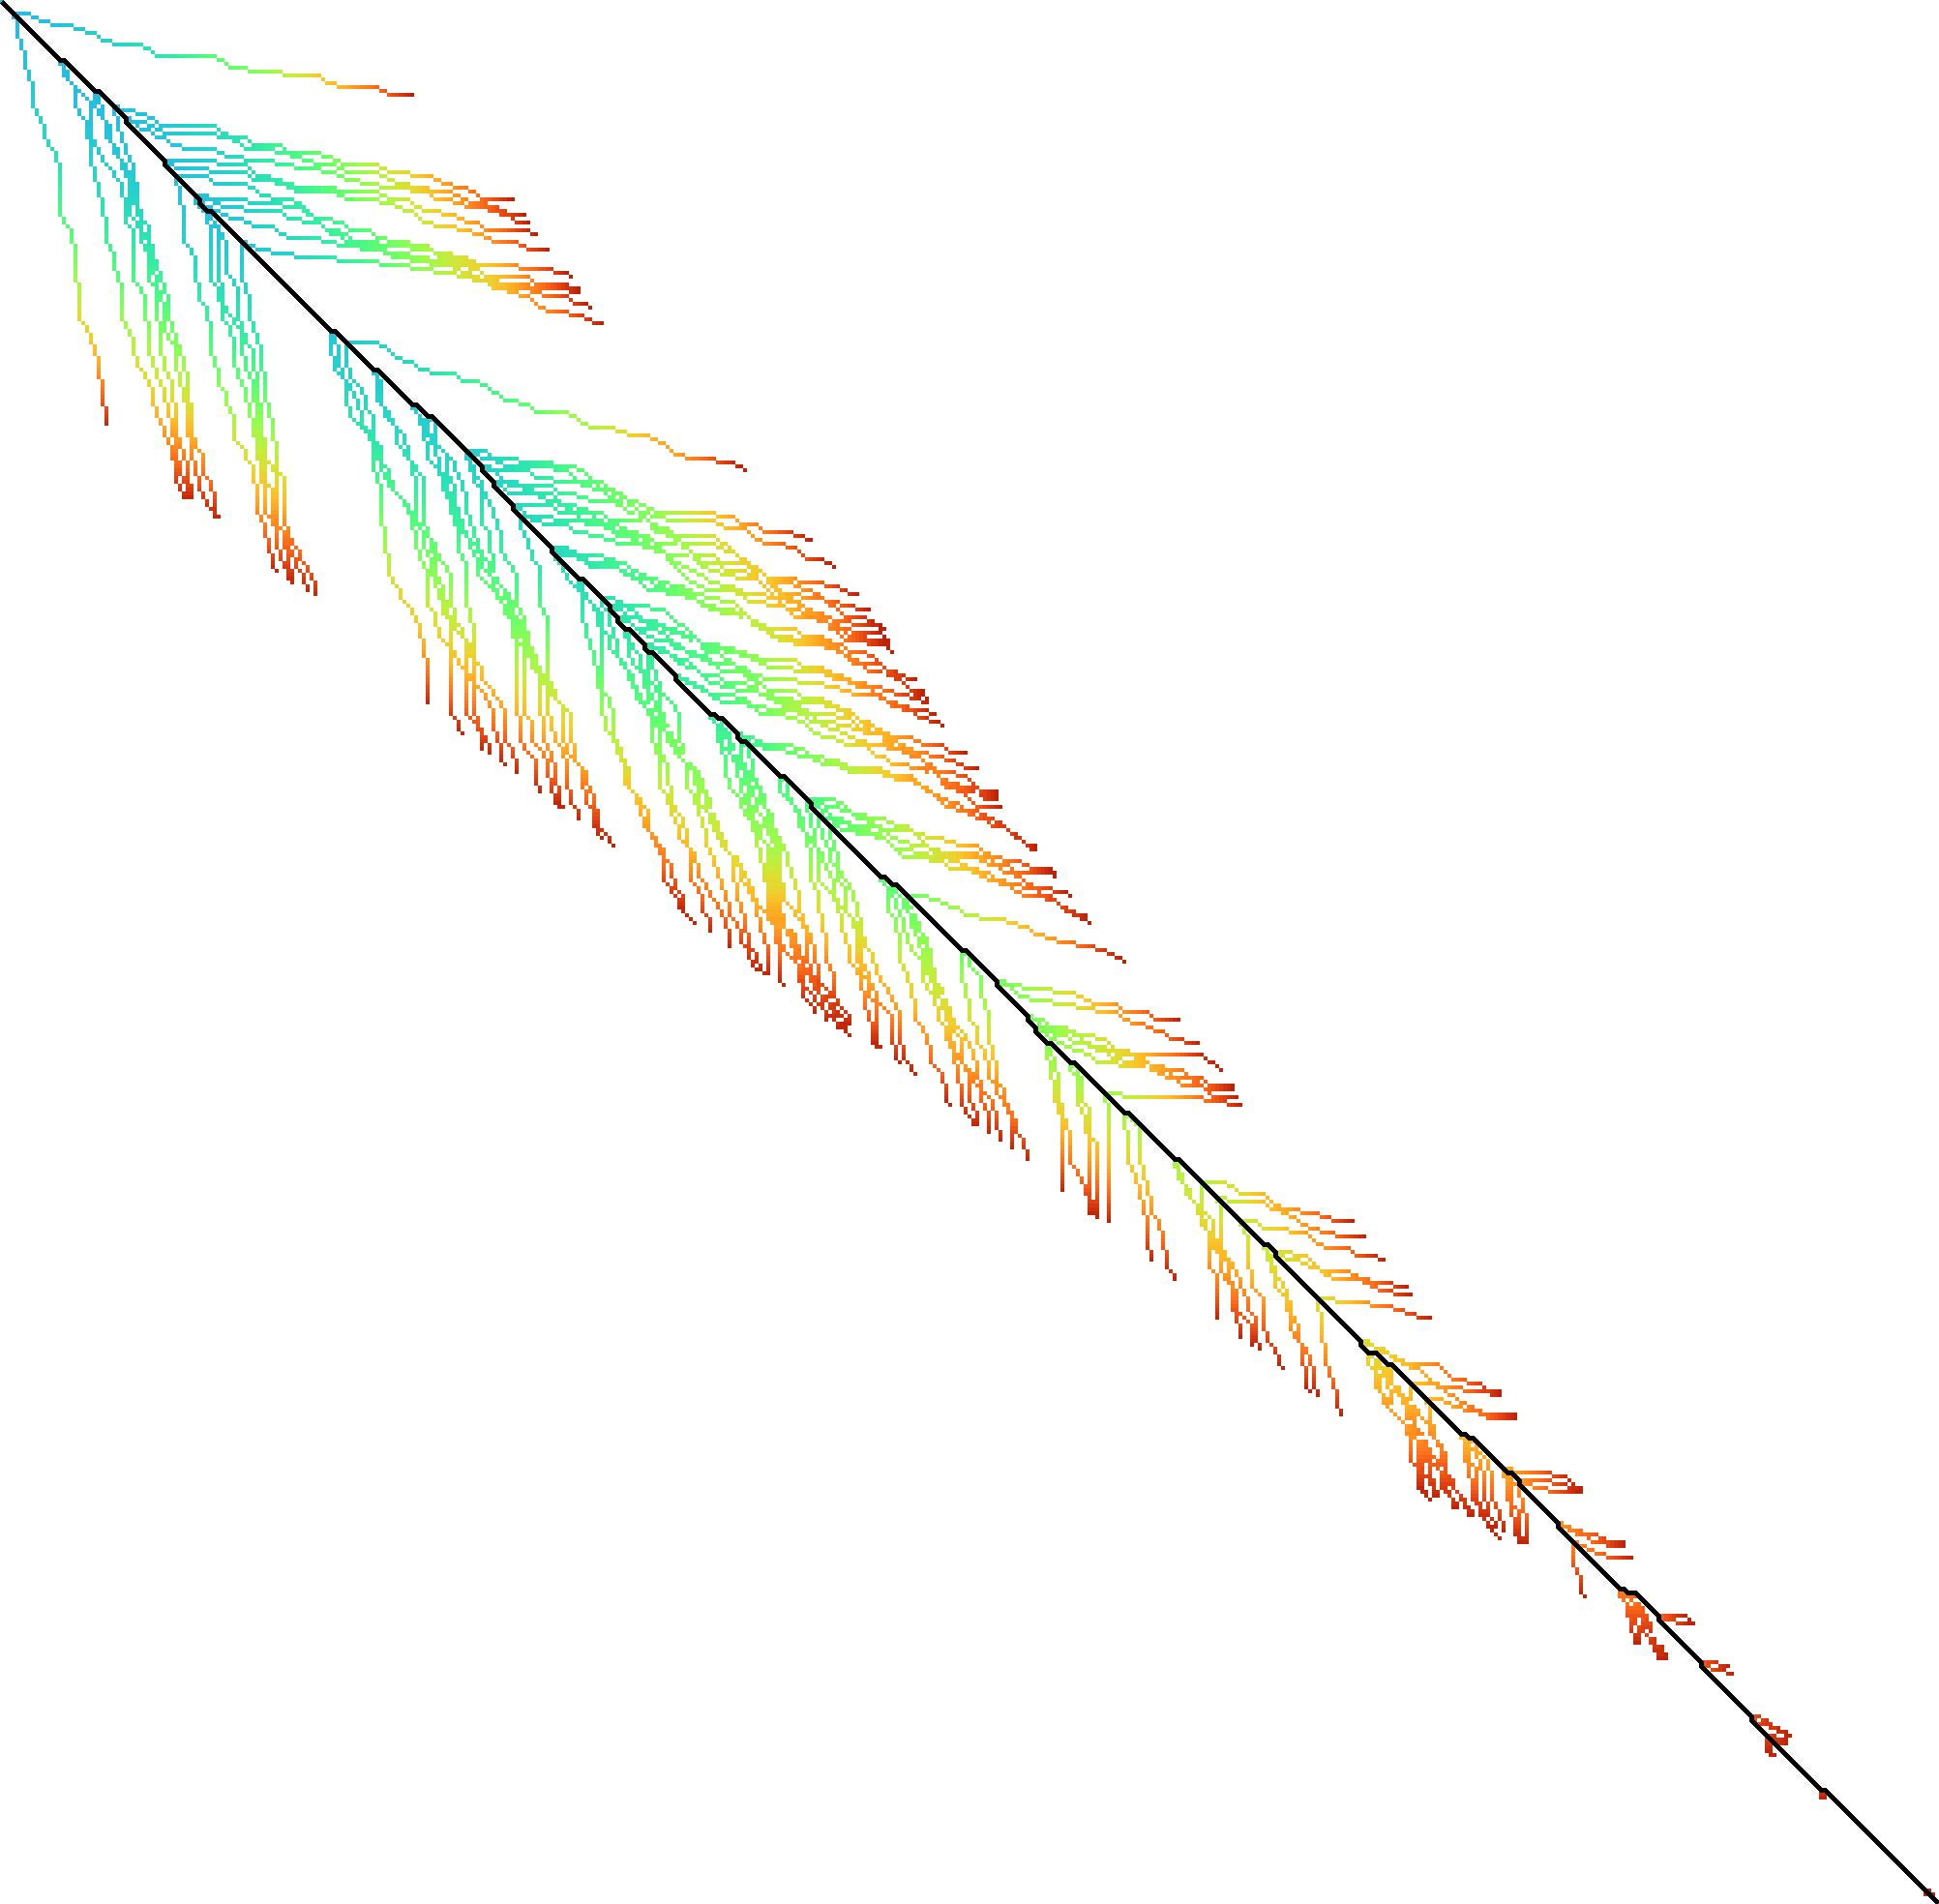
\includegraphics[width=0.33\linewidth]{imgs/intro/3_diagonal-transition.png}\label{fig1-wfa}}
    \hspace{-8em}
    \hfill
    \subfloat[\\DT+D\&C\\(\wfa)]{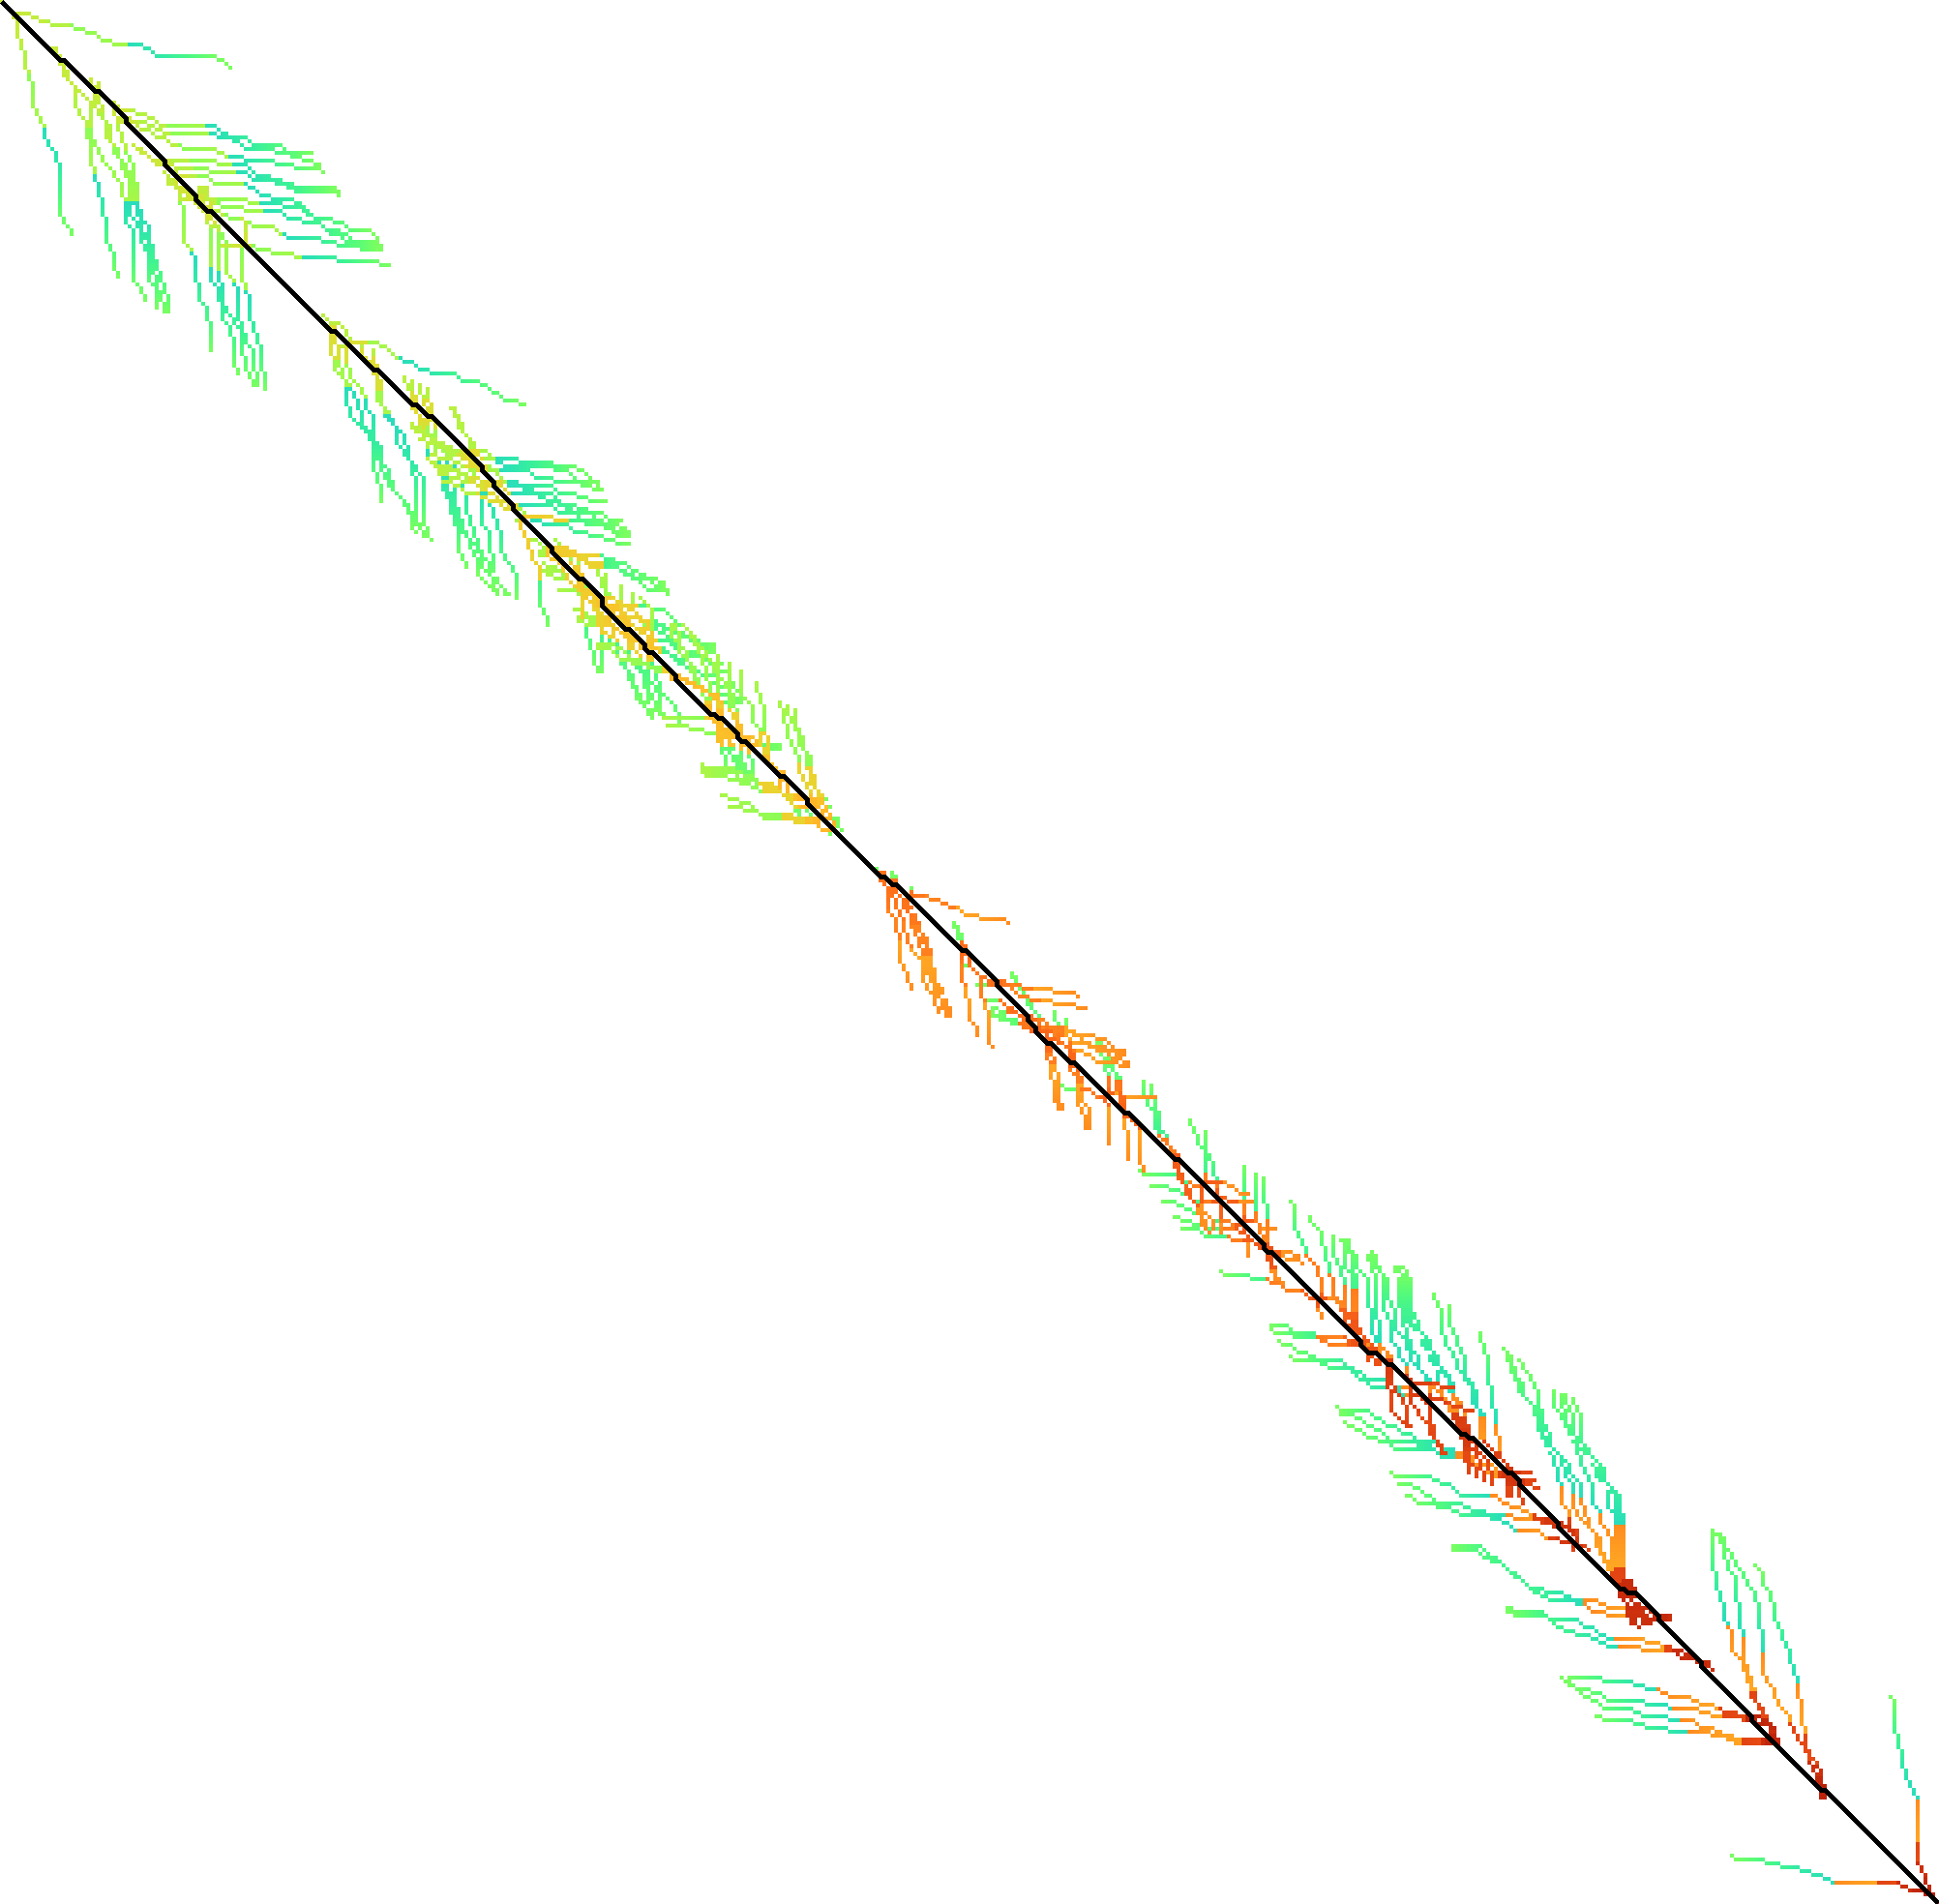
\includegraphics[width=0.33\linewidth]{imgs/intro/4_dt-divide-and-conquer.png}\label{fig1-biwfa}}
    \hspace{-8em}
    \hfill
    \subfloat[\\\textbf{This work}\\\textbf{(\astarpa)}]{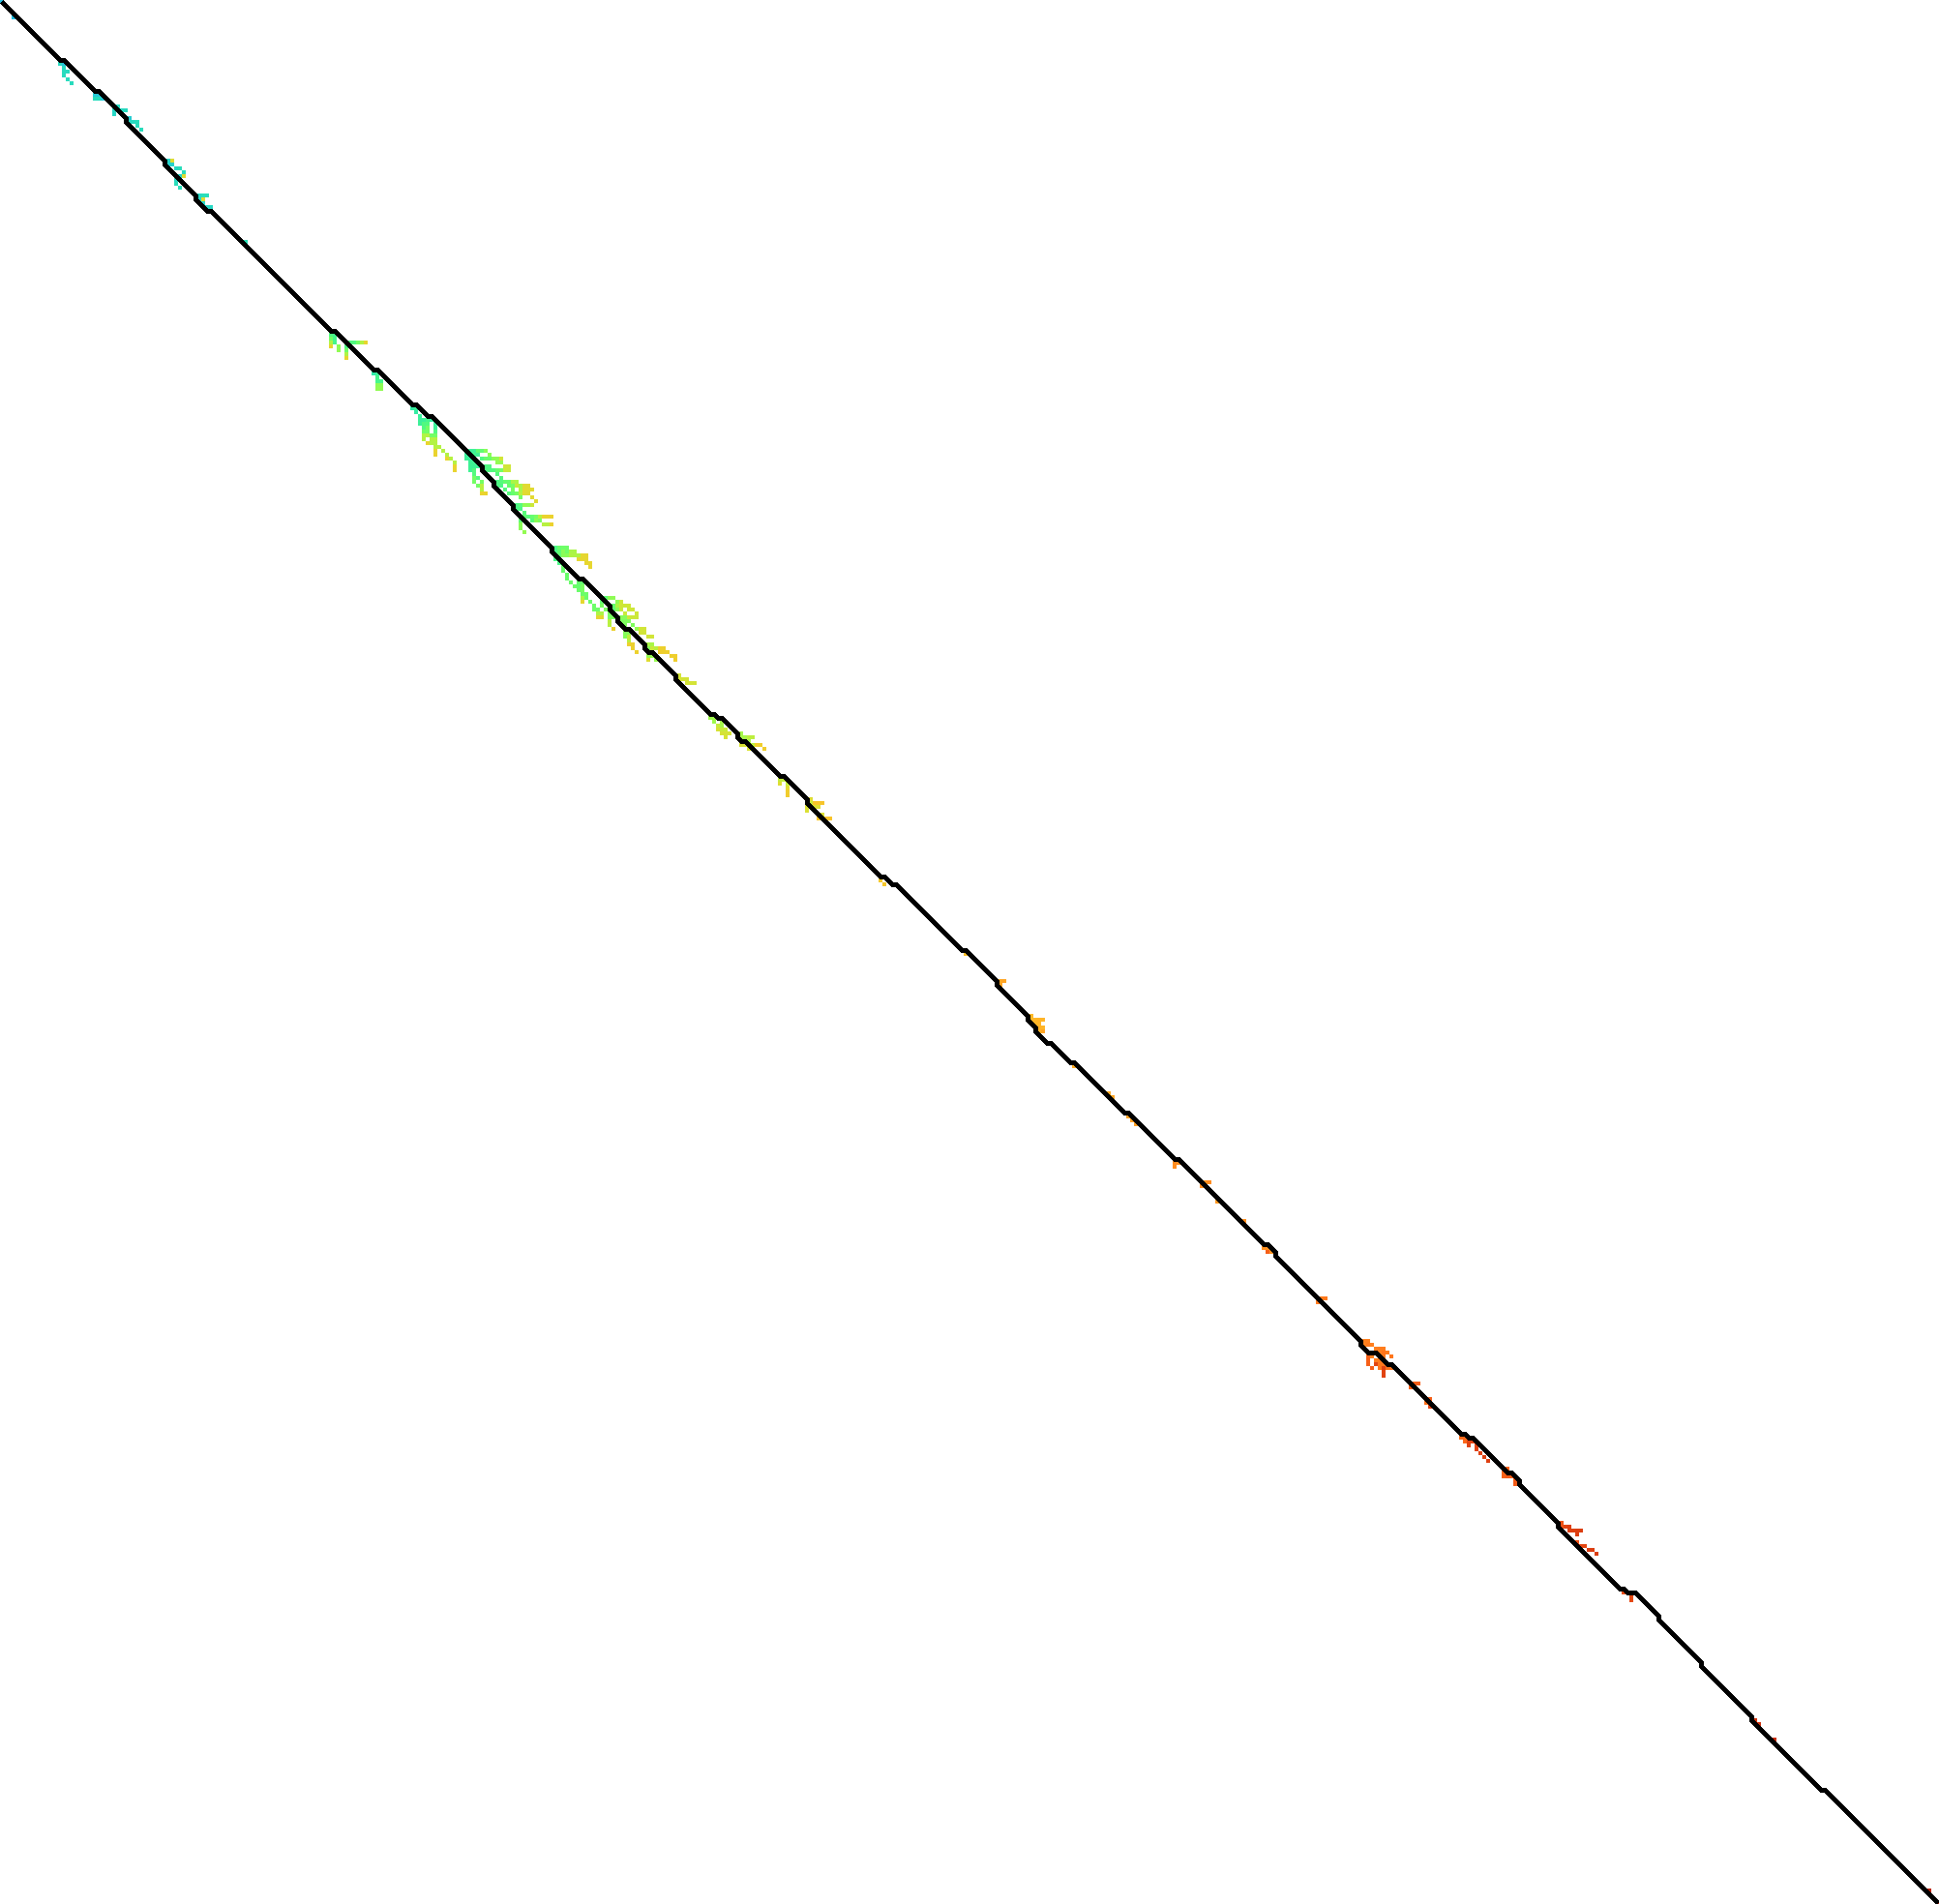
\includegraphics[width=0.33\linewidth]{imgs/intro/5_astarpa.png}\label{fig1-astar}}
    \caption{%
      \textbf{Computed states per algorithm.} Various optimal alignment
algorithms and their implementation are demonstrated on synthetic data (length
$n{=}500\bp$, divergence $d{=}16\%$). The colour indicates the order of
computation from blue to red. \protect\subref{fig1-band} Band-doubling (\edlib), \protect\subref{fig1-dij}
\dijkstra, \protect\subref{fig1-wfa} Diagonal transition/DT (\oldwfa), \protect\subref{fig1-biwfa} DT with
divide-and-conquer/D\&C (\wfa), \protect\subref{fig1-astar} \astarpa with \gch (\GCH), match
pruning, and DT (seed length $k{=}5$ and exact matches).}
    \label{fig:intro}
\end{figure}


\section{Overview}

\paragraph{Methods}
We solve exact global pairwise alignment with respect to edit distance by using
the \A shortest path algorithm on the alignment graph. In order to efficiently
align long sequences with high error rate, we extend the \emph{seed~heuristic}
with \emph{match~chaining}, \emph{inexact~matches}, and the novel
\emph{match~pruning} optimization. We prove the correctness of our algorithm and
provide an efficient implementation in \astarpa.

\paragraph{Results}
We evaluate \astarpa on synthetic data (random sequences of length $n$ with
uniform errors with rate $e$) and on real long ONT reads of human data. On the
synthetic data with $e{=}5\%$ and $n{\leq}10^7\bp$, \astarpa exhibits a
near-linear empirical runtime scaling of $n^{1.08}$ and achieves ${>}250\times$
speedup compared to the leading exact aligners \edlib and \wfa. Even for a high
error rate of $e{=}15\%$, the empirical scaling is $n^{1.28}$ for
$n{\leq}10^7\bp$. On two real datasets, \astarpa is the fastest aligner for
$58\%$ of the alignments when the reads contain only sequencing errors, and for
$17\%$ of the alignments when the reads also include biological variation.

\paragraph{Contributions}
Our algorithm exactly solves global pairwise alignment for edit distance costs,
also known as \emph{Levenshtein distance}~\citep{levenshtein1966binary}. It uses
the \A algorithm to find a shortest path in the alignment graph.

\paragraph{\Sh} In order to handle higher error rates, we extend the \emph{\sh}
to \emph{inexact matches}, allowing up to $1$ error in each match.  To handle
cases with a large number of seed matches we introduce \emph{match chaining},
constraining the order in which seed matches can be
linked~\citep{wilbur1984context,benson2016lcsk}. We prove that our \emph{\csh}
with inexact matches is admissible, which guarantees that \A finds a shortest
path.

\paragraph{Match pruning}
In order to reduce the number of states expanded by \A we apply the
\emph{multiple-path pruning} observation of \citet{poole2017artificial}: once a
shortest path to a vertex has been found, no other paths to this vertex can
improve the global shortest path. We prove that when a state at the start of a
match is expanded, a shortest path to this state has been found. Since no other
path to this state can be shorter, we show that we can \emph{prune} (remove) the
match, thus improving the \sh. This incremental heuristic search has some
similarities to Real-time Adaptive \A~\citep{koenig2006real}.

\paragraph{Implementation}
We efficiently implement our algorithm in the \astarpa aligner. In particular,
we use \emph{contours}
\citep{hirschberg1977algorithms,hunt1977fast,pavetic2017fast} to efficiently to
compute the \csh, and update them when pruning matches.

\paragraph{Scaling and performance}
We compare the scaling and performance of our algorithm to other exact aligners
on synthetic data, consisting of random genomic sequences with up to $15\%$
uniform errors and up to $10^7$ bases. We demonstrate that inexact matches and
match chaining enable scaling to higher error rates, while match pruning enables
near-linear scaling with length by reducing the number of expanded states to not
much more than the best path (\cref{GLOBALfig1-astar}). Our empirical results
show that for $e{=}5\%$ and $n{=}10^7\bp$, \astarpa outperforms the leading
aligners \edlib~\citep{vsovsic2017edlib} and \wfa~\citep{marco2022optimal} by
more than $250$ times.

We demonstrate a limited applicability of our algorithm to long Oxford
Nanopore (ONT) reads from human samples. \astarpa is the fastest exact aligner
on $58\%$ of the alignments on a dataset with only sequencing
errors, and on $17\%$ of the alignments on a dataset with biological
variation.

%\paragraph{Chaining matches} Given a set of matching substrings in the two
%sequences, the problem of connecting (\emph{chaining}) a maximal number of
%matches in increasing order in both sequences has been solved in
%$\Oh(M{\log}M)$~\citep{eppstein1992sparse,myers1992n2}.
%%\citet{myers1995chaining} Chaining of seed matches have been applied
%%by~\citep{pavetic2017fast}.

%\paragraph{Contours} \citet{hunt1977fast} developed an $\Oh((M+n) \log n)$
%algorithm using \emph{thresholds} by considering all $M$ pairs of indices of
%equal (\emph{matching}) elements in both sequences.  This is used in the
%\difftool tool \citep{hunt1976algorithm} where the sequence elements are lines
%in text files.  For nucleotide sequences where the alphabet size is small, $M$
%grows as $n^2$, leading to $\Oh(n^2 \log n)$ runtime even for similar sequences.
%%\citet{hirschberg1977algorithms} extends the concept of \emph{thresholds} to
%%\emph{dominant matches} and \emph{contours}.

%% LCSk++, Seed heuristic, possibly add myers2014efficient for seeds
%\paragraph{Seeds} \citet{benson2014longest} introduce an approach where only
%groups of $k$ consecutive letters can be matched.
%\citet{deorowicz2014efficient} extend the algorithm of \citet{hunt1977fast} to
%this setting. They first group the sequence letters into overlapping seeds of
%size $k$, effectively increasing the alphabet and hence reducing the number of
%matches $M$. Using an appropriate choise of $k$, they achieve $\Oh(n\log n)$
%expected runtime on random sequences. We use non-overlapping seeds in a
%\emph{seed heuristic} for \A to do exact semi-global alignment in the case of
%long and related sequences.